%------------------------------------------------------------------------------
%
% LaTeX-mall för examensarbeten vid LNU
% Skapad av Marcus Wilhelmsson, Institutionen för Datavetenskap
% Fakulteten för Teknik
% Linnéuniversitetet
%
% Licens: Creative Commons BY
%
% 
%------------------------------------------------------------------------------
%
%------------------------------------------------------------------------------
%	Inställningar och dokumentkonfiguration
%------------------------------------------------------------------------------

\documentclass[a4paper,12pt]{article} % A4-sida och 12 punkters fontstorlek


\usepackage[T1]{fontenc} % 8-bitarskodning som har 256 glyfer
\usepackage{times} % Typsnitt i dokumentet
\usepackage[swedish,english]{babel} % Svenskt språk, engelska för extra abstract
\usepackage[utf8]{inputenc} % För svenska tecken (UTF-8)
\usepackage{dtklogos} % Logos för t.ex. LaTeX, BibTeX, etc.
\usepackage{wallpaper} % Bakgrundsbild
\usepackage[absolute]{textpos} % Möjlighet att absolutpositionera text
\usepackage[top=2cm, bottom=2.5cm, left=3cm, right=3cm]{geometry} % Ställ in marginaler
\usepackage{appendix} % Stöd för separat hantering av bilagor
\usepackage{cite}
\usepackage{listings}
\usepackage[hidelinks]{hyperref}
\usepackage{float}


\setcounter{secnumdepth}{3} % Fem nivåer av underrubriksnumrering
\setcounter{tocdepth}{3} % Fem nivåer av underrubriksnumrering i innehållsförteckning

\usepackage{sectsty} % Ändra storlek på section och subsection till 12 punkter
\sectionfont{\fontsize{14}{15}\selectfont}
\subsectionfont{\fontsize{12}{15}\selectfont}
\subsubsectionfont{\fontsize{12}{15}\selectfont}

\usepackage{csquotes} % Används för att hantera citat


%------------------------------------------------------------------------------
%	Denna del används för att skapa boxen med författare, handledare, etc.

\newsavebox{\mybox}
\newlength{\mydepth}
\newlength{\myheight}

\newenvironment{sidebar}%
{\begin{lrbox}{\mybox}\begin{minipage}{\textwidth}}%
{\end{minipage}\end{lrbox}%
 \settodepth{\mydepth}{\usebox{\mybox}}%
 \settoheight{\myheight}{\usebox{\mybox}}%
 \addtolength{\myheight}{\mydepth}%
 \noindent\makebox[0pt]{\hspace{-20pt}\rule[-\mydepth]{1pt}{\myheight}}%
 \usebox{\mybox}}

%------------------------------------------------------------------------------
%	Titel-sektion
%------------------------------------------------------------------------------
\newcommand\BackgroundPic{
    \put(-2,-3){
    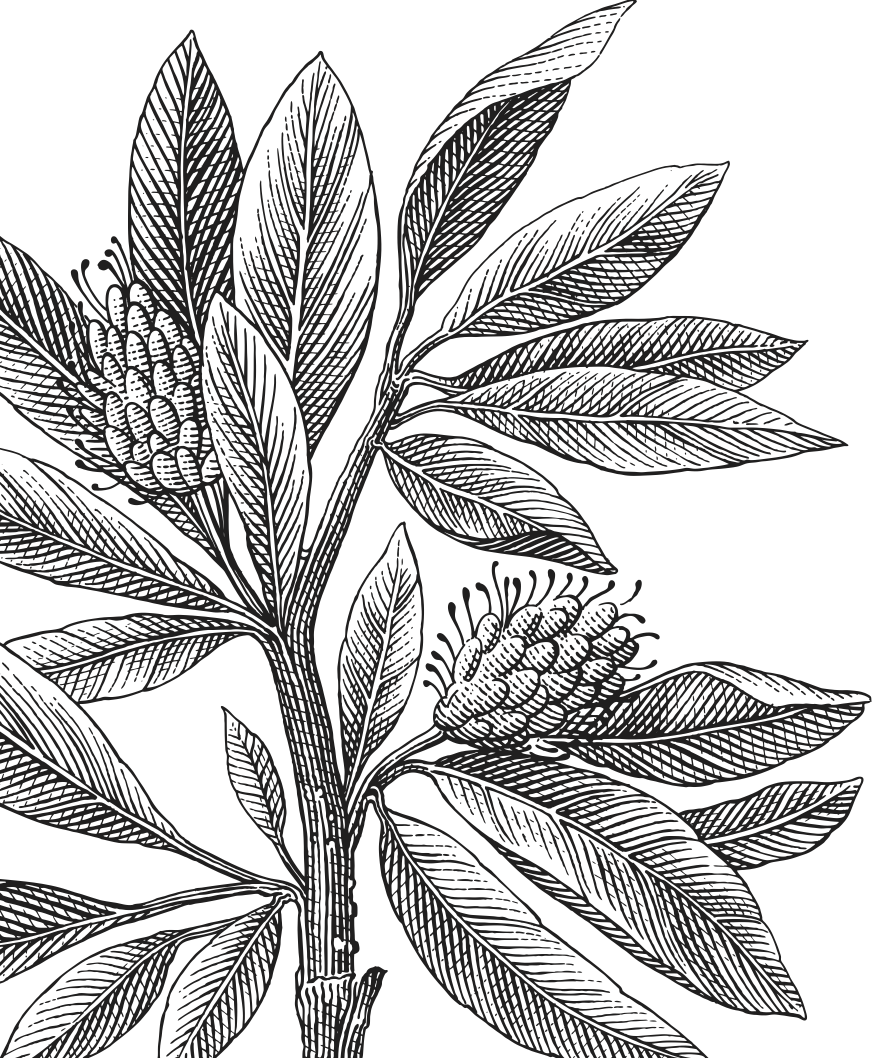
\includegraphics[keepaspectratio,scale=0.3]{img/lnu_etch.png} % Bakgrundsbild
    }
}
\newcommand\BackgroundPicLogo{
    \put(30,740){
    
\includegraphics[keepaspectratio,scale=0.10]{img/logo.png} % Logga i övre vänstra hörnet
    }
}

% In the following you can change the title of your document
\title{	
\vspace{-8cm}
\begin{sidebar}
    \vspace{10cm}
    \normalfont \normalsize
    \Huge Assignment 2\\ % Dokumentets typ, t.ex. Examensarbete
    \vspace{-1.3cm}
\end{sidebar}
\vspace{3cm}
\begin{flushleft}
    \LARGE Computer Networks - an introduction\\ % Dokumentets rubrik
 %   \it \LARGE Examensarbete under arbete % Dokumentets underrubrik
\end{flushleft}
\null
\vfill
\begin{textblock}{6}(9,11)
\begin{flushright}
\begin{minipage}{\textwidth}
\begin{flushleft} \large
\emph{Author:} John Herrlin\\ % Författare
\emph{Email: } jh222jx@student.lnu.se\\
\emph{Author:} Rasmus Sjostrom\\ % Författare
\emph{Email: } rs222kp@student.lnu.se\\
%\emph{Handledare:} Dr.~Foo \textsc{Bar}\\ % Handledare
%\emph{Examinator:} Dr.~Mark \textsc{Brown}\\ % Examinator
\emph{Semester:} VT2016\\ % Termin
\emph{Area:} Computer Science\\ % Ämne
%\emph{Level:} G2F\\ % Nivå
\emph{Coursecode:} 1DV701 % Kurskod
\end{flushleft}
\end{minipage}
\end{flushright}
\end{textblock}
}


\date{} % Dagens datum, tomt i detta fallet. Använd \today för dagens datum.

\begin{document}
\pagenumbering{gobble}
\newgeometry{left=5cm}
\AddToShipoutPicture*{\BackgroundPic} % Lägger in backgrundsbild på första sidan
\AddToShipoutPicture*{\BackgroundPicLogo} % Lägger in LNU-logga på första sidan
\maketitle % Skriv ut titeln
\restoregeometry
\clearpage
%------------------------------------------------------------------------------
%	Svensk och engelsk version av abstract
%------------------------------------------------------------------------------
{

%------------------------------------------------------------------------------
\newpage
\pagenumbering{gobble} % Stäng av sidnumrering för innehållsförteckningssidan
\tableofcontents % Innehållsförteckning
\newpage % Ny sida
\pagenumbering{arabic} % Påbörja sidnumrering på 1

%------------------------------------------------------------------------------
% This is where you write the report:
\section{Introduction}


The idea of our project was to build a small web framework, since we already
had to write the web server from scratch for the assignment. We figured this
to be a great opportunity to develop something we could continue working on
and learn more about since we consider it a very interesting field.\\
\\
Our goals with this small framework is to keep things as simple and modular
as possible, making it easy to expand or modify for further development.\\
\\
We are very well aware of the fact that the database parts were not a part
of the assignment, but to us it simply made sense to include this in the
project. Therefore, we have built a small ORM with a SQLite database found
in the db and domain modules. The reason for this was to be able to test and
use our PUT and POST methods naturally, as if we were performing them on a 
real life web server.\\
\\
We have saved the tcpclient in the code from the previous assignment.
The reson for this is that we used it for fuzzy testing against the endpoints.\\


\subsection{Workflow}

The small enumeration figure below describes the workflow of the webserver,
starting with a request and ending with a response being sent back.

\begin{enumerate}
  \item Parse an incoming request and create a Request object
  \item Send the request object to the URL handler, which will match the Request.uri with specified patterns
  \item If the requested uri matches a pattern, the URL handler will call the corresponding View, forward the request as an argument
  \item Depending on the called view, proper business logic will be executed. Thereon a response and body will be sent back to the client
\end{enumerate}
\\
By following this model, adding new URLs and a corresponding View for that URL is extremely easy.

\section{Problem 1}

\begin{figure}[H]
    \centering  
    
\includegraphics[scale=0.5]{img/screenshots/htmlindex.png}
	\label{fig:htmlindex}
	\caption{Index page with imgs and CSS.}
\end{figure}


\begin{figure}[H]
    \centering  
    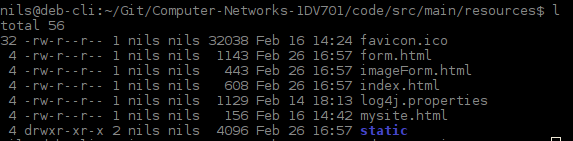
\includegraphics[scale=0.5]{img/screenshots/filesresourcefolder.png}
	\label{fig:filesresourcefolder}
	\caption{Resource folder, site root.}
\end{figure}


\begin{figure}[H]
    \centering  
    
\includegraphics[scale=0.6]{img/screenshots/htmlstatic.png}
	\label{fig:htmlstatic}
	\caption{HTML document in static folder.}
\end{figure}



\section{Problem 2}

The table in ~\ref{fig:responsecodesandusage} describes different types of response codes that the server sends back to the client.
We table describes response codes that are both in the G task in Problem 1 and VG-task 1 in Problem 2.
The reason to have everything in one table and not to split them up if for the simplicity and readability.

\begin{figure}[H]

  \begin{tabular}{ | l | l | }
    \hline			
    Code & Usage \\
    \hline			
    200 & OK, Many places where server handles response in a correct way. \\
    \hline			
    201 & Created, When success with POST on /post Figure~\ref{fig:response201created} \\
    \hline			
    202 & Accepted, When /login success Figure~\ref{fig:response202login} \\
    \hline			
    205 & Reset Content, When /logout success. Figure~\ref{fig:response205logout} \\
    \hline			
    400 & Bad Request, When NOT PUT on /put . Figure~\ref{fig:response400put} \\
    \hline			
    403 & Forbidden, When trying trying /post or /put but have not logged in (/login) before Figure~\ref{fig:response403forbidden} \\
    \hline			
    404 & Not Found, When trying to access a static file but cant find it OR if url doesn match any Figure~\ref{fig:response404notfound} \\
    \hline			
    405 & Method Not Allowed, When NOT POST on /post Figure~\ref{fig:response405methodnotallowed} \\
    \hline			
    500 & Server Error, If we cant parse the request Figure~\ref{fig:response500servererror} \\
    \hline  
  \end{tabular}
  \label{fig:responsecodesandusage}
  \caption{Response codes and their usage.}
\end{figure}

\section{Screenshots}

hey 

\begin{figure}[H]
    \centering  
    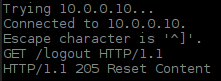
\includegraphics[scale=1]{img/screenshots/response205logout.png}
	\label{fig:response205logout}
	\caption{Method: GET, Endpoint: /logout, Response: 205 Reset Content}
\end{figure}

hey 

\begin{figure}[H]
    \centering  
    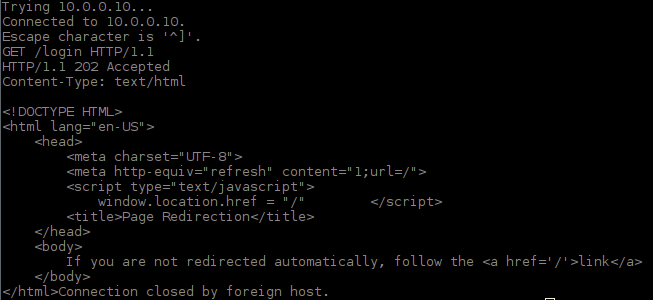
\includegraphics[scale=0.6]{img/screenshots/response202login.png}
	\label{fig:response202login}
	\caption{Method: GET, Endpoint: /login, Response: 202 Accepted}
\end{figure}

hey 

\begin{figure}[H]
    \centering  
    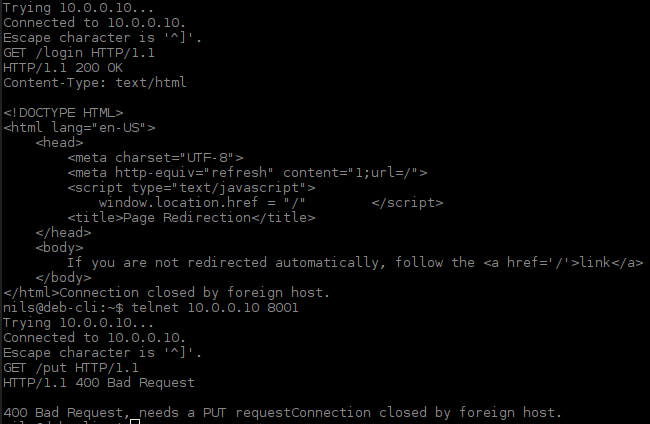
\includegraphics[scale=1]{img/screenshots/response400put.png}
	\label{fig:response400put}
	\caption{Method: GET, Endpoint: /put, Response: 400 Bad Request}
\end{figure}

hey 

\begin{figure}[H]
    \centering  
    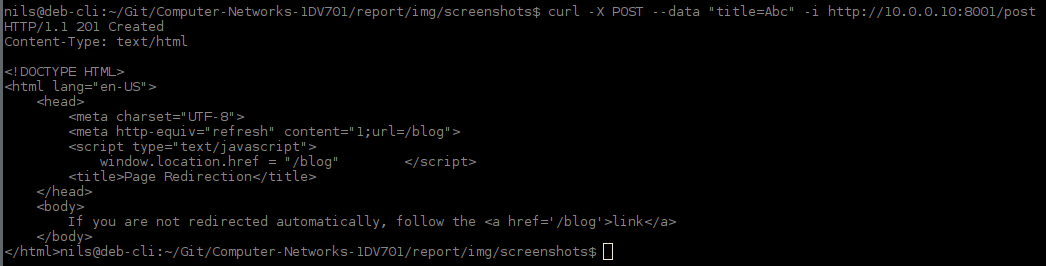
\includegraphics[scale=0.40]{img/screenshots/response201created.png}
	\label{fig:response201created}
	\caption{Method: POST, Endpoint: /post, Response: 201 Created}
\end{figure}


\begin{figure}[H]
    \centering  
    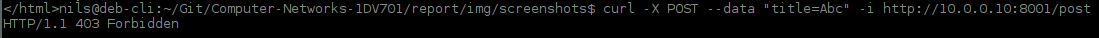
\includegraphics[scale=0.40]{img/screenshots/response403forbidden.png}
	\label{fig:response403forbidden}
	\caption{Method: POST, Endpoint: /post, Response: 403 Forbidden}
\end{figure}

\begin{figure}[H]
    \centering  
    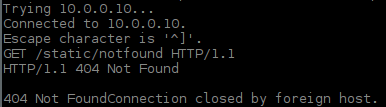
\includegraphics[scale=0.70]{img/screenshots/response404notfound.png}
	\label{fig:response404notfound}
	\caption{Method: GET, Endpoint: /static/notfound, Response: 404 Not Found}
\end{figure}

hejsa

\begin{figure}[H]
    \centering  
    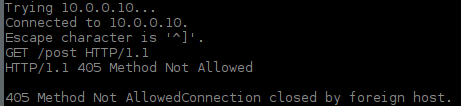
\includegraphics[scale=0.70]{img/screenshots/response405methodnotallowed.png}
	\label{fig:response405methodnotallowed}
	\caption{Method: GET, Endpoint: /post, Response: 405 Method Not Allowed}
\end{figure}

\begin{figure}[H]
    \centering  
    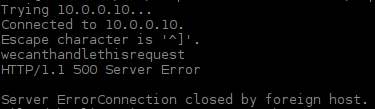
\includegraphics[scale=0.80]{img/screenshots/response500servererror.png}
	\label{fig:response500servererror}
	\caption{Method: ?, Endpoint: ?, Response: 500 Server Error}
\end{figure}


\section{How To Run/Build}

The application can be run from the TCPserver -> ServerThread class, located in
the TCP module. The required arguments to run the server is '-m tcpserver'

%------------------------------------------------------------------------------
%\bibliographystyle{IEEEtran}
% Here you will have to put your bibliography
%% \newpage
%% \bibliography{ieeedb.bib}{}
%% \bibliographystyle{IEEEtran}


\end{document}
